% Development

% Main chapter title
%\chapter[toc version]{doc version}
\chapter{Development}

% Short version of the title for the header
%\chaptermark{version for header}

% Chapter Label
% For referencing this chapter elsewhere, use \ref{ChapterTemplate}
\label{Development}

This chapter describes the development of the timetable system, formulating the problem, discussing the implementation of the \ac{mcts} and \ac{hc} hybrid approach, detailing the design choices, algorithmic improvements and integration efforts made throughout the project.

\section{Search Space}

The search space, \(S\),  for this problem is large as it involves a product of all possible event-period-room combinations: \[S = E \cdot P  \cdot R,\] where \(E\) is the set of events, \(P\) is the set of periods (day,timeslot), and \(R\) is the set of rooms.

\section{Problem Formulation}

(...)
The entities in the problem are listed below:

\begin{itemize}
	\item \textbf{Periods, \(P = \{P_1, P_2, ..., P_|_P_|\}\):} Days are divided into fixed timeslots, with periods consisting of a day and a timeslot.

		\unsure[inline]{In the previous work, there is no periods. There are weekdays, a start time and an end time. For now, in the current approach, an event is only associated with a period of one hour and without any link to previous work. If I implement this concept to previous work, an event should be assigned to one or more half-hour periods.}

	\item \textbf{Rooms, \(R = \{R_1, R_2, ..., R_|_R_|\}\):} Each room has a capacity and a type.
		\begin{itemize}
			\item Occupation (the room may be utilized for non-teaching reasons, such as exams) (TODO)
			\item Capacity (number of seats)
			\item Type (TODO)
		\end{itemize}

	\item \textbf{Lecturers, \(L = \{L_1, L_2, ..., L_|_L_|\}\):} 
		\begin{itemize}
			\item Office
			\item Restriction (availability and TODO: preferences for periods)
		\end{itemize}

	\item \textbf{Events, \(E = \{E_1, E_2, ..., E_|_E_|\}\):} Represent the events to be scheduled. Each event has associated attributes:
		\begin{multicols}{2}
		\textbf{Previous work:}
		\begin{itemize}
			\item Start and end time
			\item Weekday
			\item Duration
			\item Lecturer
			\item Room
		\end{itemize}
		\columnbreak
		\textbf{TODO: adicionar ao trabalho anterior?}
		\begin{itemize}
			\item Period
        		\item Capacity (number of students)
        		\item Number of lectures
        		\item Minimum working days (days over which the events of the same block should be spread)
        		\item Available periods
        		\item Priority
		\end{itemize}
		\end{multicols} 

	\item \textbf{Blocks, \(B = \{B_1, B_2, ..., B_|_B_|\}\):} A block may represent a group of related events, such as all events of a subject, or events from the same course and curricular year.
\end{itemize}

\subsection{Constraints}

There are several hard and soft constraints that affect the creation of \ac{fcup} timetables. The following hard and soft constraints were selected, drawing inspiration from those of \ac{itc-2007}:

\textbf{Hard constraints:}

\begin{itemize}
	\item \textbf{H1:} Events belonging to the same subject must be scheduled and must be assigned to distinct periods.
	\item \textbf{H2:} Two events can be scheduled in the same room, but only if they are in different periods.
	\item \textbf{H3:} Events of the same course and curricular year, or taught by the same lecturer, must be scheduled in different periods.
	\item \textbf{TODO H4:} If a room is unavailable in a given period, then no events can be scheduled in that period.
	\item \textbf{H5:} If a lecturer is unavailable in a given period, then no events can be taught by this lecturer in that period.
	\item \textbf{TODO H6:} Lecturers and students must have a free lunch period.
\end{itemize}

\textbf{Soft constraints:}

\begin{itemize}
	\item \textbf{S1:} Events of the same subject should be spread into the given minimum number of days.
	\item \textbf{S2:} Events belonging to the same course and curricular year should be in consecutive periods.
	\item \textbf{S3:} The capacity of the room should be higher or equal than the capacity of the event.
	\item \textbf{S4:} All events of a subject should be given in the same room.
\end{itemize}


%Maximization problem...

\section{Monte Carlo Tree Search}

%This section describes the key algorithmic components of the system, particularly the hybrid \ac{mcts} with \ac{hc} approach.

(...)

\subsection{\ac{mcts} Tree}

\begin{figure}
      \centering
      \includegraphics[width=0.6\columnwidth]{Development/MCTS_tree.jpg}
      \caption[MCTS tree]
      {MCTS tree}
      \label{fig:mcts_tree}
\end{figure}

Figure \ref{fig:mcts_tree} illustrates the basic structure of the \ac{mcts} tree. The root represents the initial state, where no events have been assigned. The first level corresponds to assigning the first event, \(E1\), to various \(P\) and \(R\). Each child node represents a specific assignment (\((E_1,P_1,R_1),...,(E_1,P_|_P_|,R_|_R_|)\)). Subsequent levels correspond to the sequential assignment of events \(E_2, E_3, ..., E_|_E_|\). Unavailable periods are discarded immediately to reduce the search space.

The events are sorted in advance so that the most difficult event to place is placed first in the tree. The priority of an event (Formula \ref{priority}) is calculated based on:
\begin{itemize}
\item The difference between the number of lectures and minimum working days to prioritize events with more lectures spread over fewer days;
\item The number of available periods, as having more available periods indicates fewer scheduling restrictions;
\item The capacity of an event, which implies that events with greater capacity have higher priority;
\item The number of blocks in which the event is, as events that appear in more blocks are more difficult to allocate.
\end{itemize}

\begin{equation}
  \begin{aligned}
	Priority = (\#lectures - \#min\_working\_days) \cdot 4 \\
	           - \#available\_periods \cdot 3 \\
	          + capacity \cdot 2 \\
	          + \#blocks\label{priority}
  \end{aligned}
\end{equation}

%I have tried other priority formulas...

\subsubsection{Tree Nodes}

A node is composed of the following attributes:

\begin{itemize}
\item A \textbf{path} is a dictionary that represents the sequence of actions leading to a node. The root is the only node that has an empty path.

\item A \textbf{parent} is a reference to the parent node, allowing the tree structure to be navigated upwards. The root is the only node that does not have a parent.

\item \textbf{Children} is initialized as an empty list at first but will later hold references to the node's child nodes. 

\item The \textbf{expansion limit} specifies the maximum number of children that a node can have, which helps control the expansion process. It is estimated based on the number of available rooms per period for the next event. A value of zero indicates that the node cannot be expanded further.

\item \textbf{Visits} is initialized to 0, tracking the number of times a node has been visited.

\item The \textbf{hard and soft scores} are both initialized to 0, representing the cumulative hard and soft scores for a node, which are used to evaluate the quality of the node's state.

\item The \textbf{best hard and soft penalty results} are initialized to negative infinity, representing the best hard and soft penalty results encountered for a node. These attributes will be updated during the algorithm as better results are found. 
\end{itemize}

\subsection{Methodology}

Figure \ref{fig:mcts_steps}(...)

\begin{figure}[H]
      \centering
      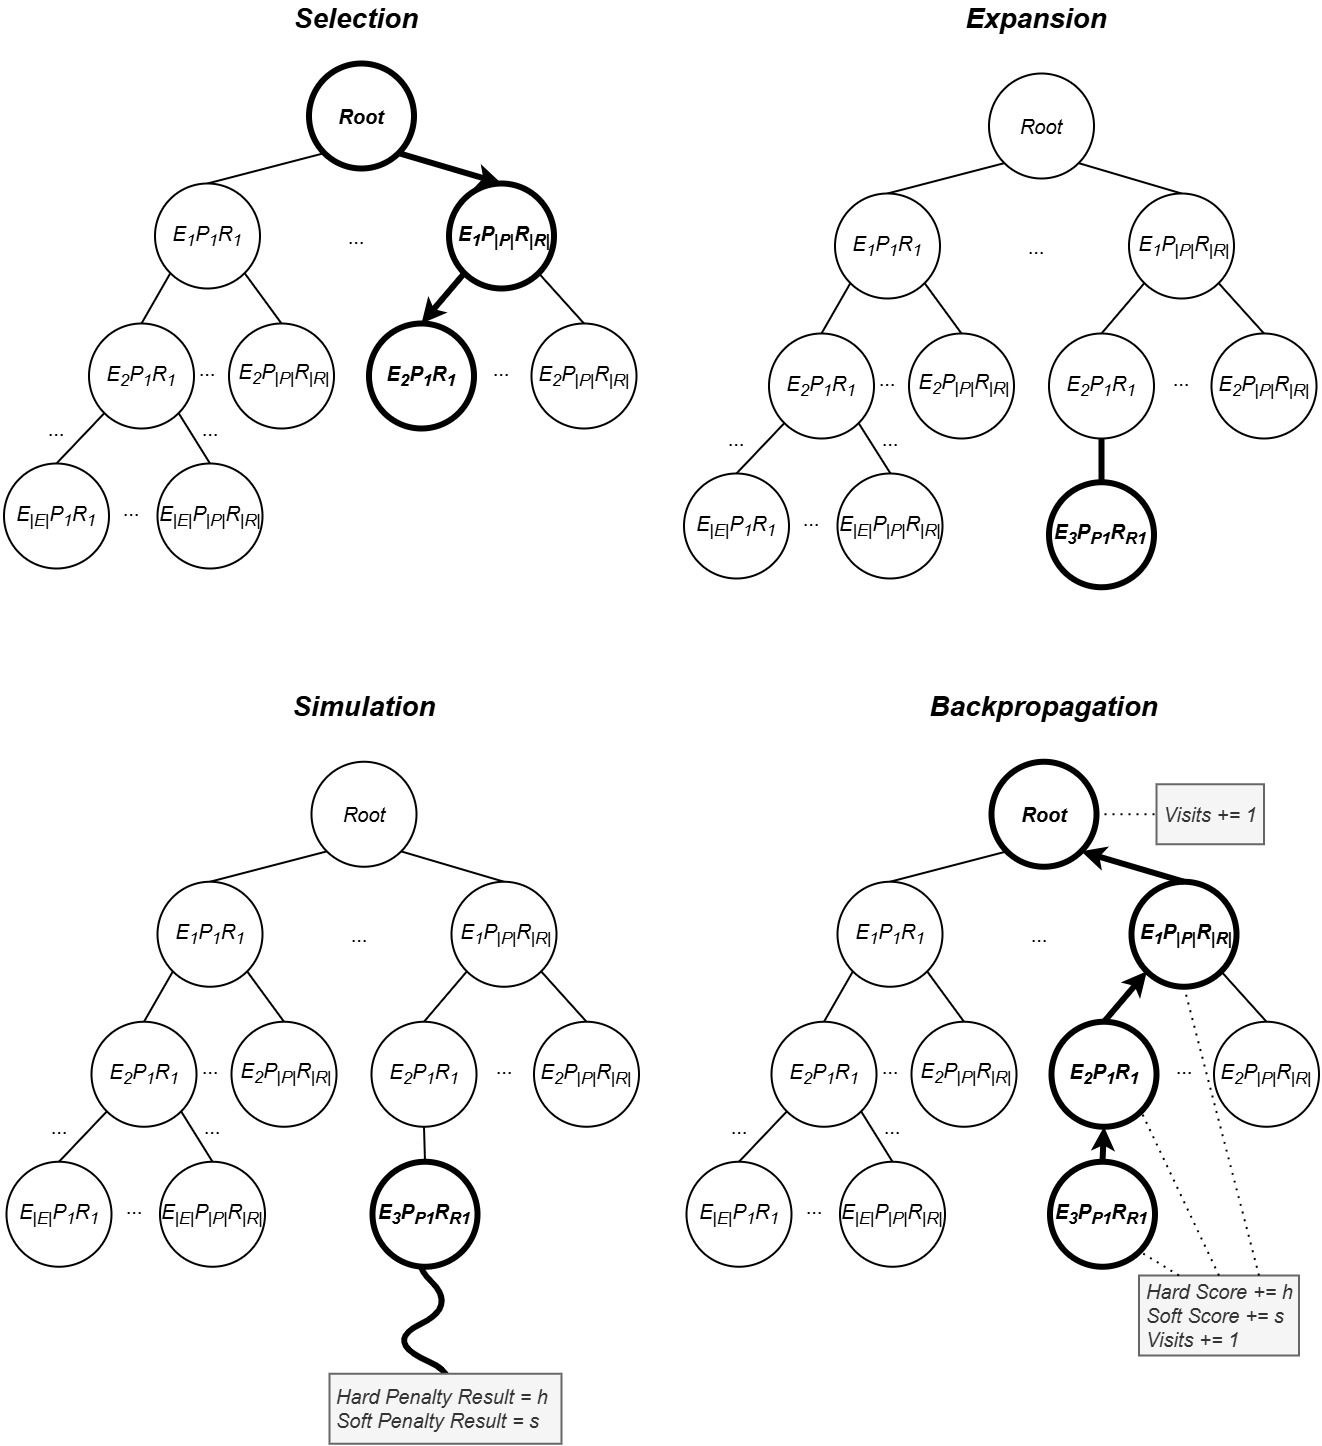
\includegraphics[width=\columnwidth]{Development/MCTS_steps.jpg}
      \caption[MCTS steps]
      {MCTS steps}
      \label{fig:mcts_steps}
\end{figure}

\subsubsection{Selection}

The \(selection\) phase (Algorithm \ref{selection}) begins at the root and traverses the tree by iteratively selecting the best child nodes until a terminal (leaf) node is reached. A node is considered terminal if either it cannot be expanded further (i.e., its expansion limit is zero) or if it has reached the maximum depth (i.e., all the events have been assigned). Conversely, a node is deemed fully expanded if either its expansion limit is zero or if the number of its children equals its expansion limit. When the traversal encounters a node that is not fully expanded, the process stops, and that node is selected for further expansion.

The best child node (Algorithm \ref{best_child}) is determined by applying the \ac{uct} formula (\ref{uct_formula}). However, as the problem has two goals, maximizing the hard constraints first and then the soft constraints, the \ac{uct} formula was applied differently. Initially, the algorithm computes the weights for each child node using the hard score. Among the children with the highest hard score, the weights are recalculated based on the soft score. The child node with the highest weight in this second calculation is selected as the best child. However, if all of a node's children have reached their expansion limit, the algorithm backtracks: if the current node has a parent, the current node expansion limit is set to zero, and it moves up to the parent. Reaching the root indicates that the entire tree is fully expanded.

\begin{algorithm}
\caption{Selection}\label{selection}
\begin{algorithmic}[1]
\Procedure{SELECTION}{}
    \State current\_node $\gets$ root
    \While{not current\_node.\textit{is\_terminal\_node}(\textit{len}(events))}
        \If{not current\_node.\textit{is\_fully\_expanded}()}
            \State \textbf{break}
        \EndIf
        \State unflagged\_children $\gets$ [child \textbf{for each} child \textbf{in} current\_node.children \textbf{if} child.expansion\_limit $\neq$ 0]
        \If{unflagged\_children is empty}
            \If{current\_node.parent exists}
                \State current\_node.expansion\_limit $\gets 0$
                \State current\_node $\gets$ current\_node.parent
            \Else
                \State \Return False
            \EndIf
        \Else
            \State best\_child $\gets$ current\_node.\textit{best\_child}(unflagged\_children)
            \State current\_node $\gets$ best\_child
        \EndIf
    \EndWhile
    \State self.current\_node $\gets$ current\_node
    \State \Return True
\EndProcedure
\end{algorithmic}
\end{algorithm}

\begin{algorithm}
\caption{Best Child}\label{best_child}
\begin{algorithmic}[1]
\Function{BEST\_CHILD}{unflagged\_children, c\_param = 1.4}
    \State choices\_weights $\gets$ [child.score\_hard $+$ c\_param $\cdot \sqrt{\frac{2\ln(\textit{self.visits})}{child.visits}}$ \textbf{for each} child \textbf{in} unflagged\_children]
    \\
    \State max\_weight $\gets$ \textit{max}(choices\_weights)
    \State best\_children $\gets$ [unflagged\_children[i] \textbf{for each} i, weight \textbf{in} \textit{enumerate}(choices\_weights) \textbf{if} weight = max\_weight]
    \\
    \State choices\_weights $\gets$ [child.score\_soft $+$ c\_param $\cdot \sqrt{\frac{2\ln(\textit{self.visits})}{child.visits}}$ \textbf{for each} child \textbf{in} best\_children]
    \\
    \State \Return best\_children[\textit{index\_of}(\textit{max}(choices\_weights))]
\EndFunction
\end{algorithmic}
\end{algorithm}

\subsubsection{Expansion}

The \(expansion\) phase (Algorithm \ref{expansion}) is responsible for expanding the node previously selected by adding a new child node. It starts by retrieving the next unvisited event based on the current node's depth, which is the length of its path. 

The algorithm also retrieves the corresponding weekday and timeslot and finds the available rooms per period for the event (Algorithm \ref{find_available_rooms}), removing occupied rooms and filtering rooms based on capacity. If rooms are available, it selects the corresponding one and creates a new event with the selected room, weekday, and timeslot. After this selection, the expansion limit for the next event in the timetable is estimated, i.e., the number of children that the new current node child will probably have. If no more events remain, the limit is set to zero. Otherwise, it sums the number of available rooms per period for the next event.
 
Finally, a new child node is created and added to the tree. The current node is updated to this newly created node.

\begin{algorithm}
\caption{Expansion}\label{expansion}
\begin{algorithmic}[1]
\Procedure{EXPANSION}{}
    \State event $\gets$ events[current\_node.\textit{depth}()]
    \State available\_periods $\gets$ event["Available\_Periods"]
    \\
    \State period $\gets$ \textit{len}(current\_node.children)
    \State period\_index $\gets$ period \% \textit{len}(available\_periods)
    \State new\_weekday, new\_timeslot $\gets$ available\_periods[period\_index]
    \\
    \State available\_rooms $\gets$ \textit{find\_available\_rooms}()
    \\
    \State new\_room\_index $\gets$ period // \textit{len}(available\_periods) \% \textit{len}(available\_rooms)
    \State new\_room $\gets$ available\_rooms[new\_room\_index]
    \\
    \State new\_path $\gets$ \textit{copy}(current\_node.path)
    \State new\_path[event["Id"]] $\gets$ \{**event, "RoomId": new\_room, "WeekDay": new\_weekday, "Timeslot": new\_timeslot\}
    \\
    \State next\_event $\gets$ events[current\_node.\textit{depth}()+1] \textbf{if} current\_node.\textit{depth}() + 1 $<$ \textit{len}(events) \textbf{else} None
    \\
    \If {next\_event is None}
         \State expansion\_limit $\gets$ 0
    \Else
         \State expansion\_limit $\gets$ \textit{sum}\big( \textit{len}(rooms) \ \textbf{for each} rooms \ \textbf{in} \textit{find\_available\_rooms}() \big)
    \EndIf
    \\
    \State child\_node $\gets$ MCTSNode(expansion\_limit = expansion\_limit, parent = current\_node, path = new\_path)
    \State current\_node.children.\textit{append}(child\_node)
    \State current\_node $\gets$ child\_node
\EndProcedure
\end{algorithmic}
\end{algorithm}



\begin{algorithm}
\caption{Find Available Rooms}\label{find_available_rooms}
\begin{algorithmic}[1]
\Function{FIND\_AVAILABLE\_ROOMS}{event\_capacity, rooms, events, available\_periods}
    \State period\_room\_availability $\gets$ \{period: \textit{set}(rooms.keys()) \textbf{for each} period \textbf{in} available\_periods\}
    \\
    \For{\textbf{each} other\_event \textbf{in} events}
        \State occupied\_period $\gets$ (other\_event["WeekDay"], other\_event["Timeslot"])
        \If{occupied\_period \textbf{in} period\_room\_availability}
            \State period\_room\_availability[occupied\_period].\textit{discard}(other\_event["RoomId"])
        \EndIf
    \EndFor
    \\
    \State suitable\_rooms $\gets$ \{room\_id \textbf{for each} room\_id, room \textbf{in} rooms.items() \textbf{if} room["Capacity"] $\geq$ event\_capacity\}
    \\
    \For{\textbf{each} period \textbf{in} available\_periods}
        \If{period\_room\_availability[period] is not empty}
            \State period\_room\_availability[period] $\gets$ period\_room\_availability[period] $\cap$ suitable\_rooms 
            \State \textbf{if empty:} keep original period\_room\_availability[period]
        \EndIf
    \EndFor
    \\
    \State \Return period\_room\_availability
\EndFunction
\end{algorithmic}
\end{algorithm}

\subsubsection{Simulation}

The simulation phase estimates the value of multiple actions, in this case, distinct event allocations, which will guide the selection and expansion steps in future iterations. 

A random event allocation approach was initially explored but produced suboptimal results. Therefore, a more structured method was implemented.

The \(simulation\) phase starts by creating a copy of the current node's path, which contains the events already scheduled. It then identifies the remaining events, i.e., events that have not been assigned yet. These remaining events are sorted based on two criteria:
\begin{enumerate}
\item Whether they were previously unassigned in prior simulations, to prioritize harder-to-schedule events.
\item Their priority, ensuring that more critical events are allocated first.
\end{enumerate}

For each unvisited event, the best available period and room combination is sought. The approach is similar to constraint programming as it iterates through all the available periods and rooms, calculating the hard and soft penalties for each combination. The combination with no hard penalties and the lowest soft penalty is selected as the best option. If multiple optimal choices exist, one is randomly selected. The event is then updated with the selected room, weekday, and timeslot. If no valid allocation is found, the event will have higher priority in the next simulation.

After scheduling all events, the simulation result is calculated, and the best and worst penalty scores are then updated based on these results. If a new best result is found, the timetable is saved to a file. If a new best result is found and the hard penalty is zero, indicating a feasible solution, the \ac{hc} algorithm (section \ref{hill_climbing_section}) is used to further optimize the timetable.

\begin{algorithm}
\caption{Simulation}\label{simulation}
\begin{algorithmic}[1]
\Function{SIMULATION}{start\_time, time\_limit}
    \State assigned\_events $\gets$ current\_node.path.\textit{copy}()
    \State unassigned\_events $\gets$ \textit{set}()
    \State remaining\_events $\gets$ \textit{sorted}(events[current\_node.\textit{depth}():], 
    \Statex \hspace{3cm} \textbf{key} = $\lambda$ event: (event["Id"] \textbf{in} previous\_unassigned\_events, event["Priority"], \textit{random.random()}), 
    \Statex \hspace{3cm} \textbf{reverse} = True)
    \\
    \For{\textbf{each} $i, event$ \textbf{in} \textit{enumerate}(remaining\_events)}
        \State best\_room\_and\_period $\gets$ \textit{find\_best\_room\_and\_period}()
        \If{best\_room\_and\_period exists}
            \State event["RoomId"], event["WeekDay"], event["Timeslot"] $\gets$ best\_room\_and\_period
            \State assigned\_events[event["Id"]] $\gets$ event
        \Else
            \State previous\_unassigned\_events.\textit{add}(event["Id"])
            \State unassigned\_events.\textit{add}(event["Id"])
        \EndIf
    \EndFor
    \\
    \State hard\_penalty\_result, soft\_penalty\_result $\gets$ \textit{evaluate\_timetable}(assigned\_events, unassigned\_events)
    \\
    \State current\_hard\_values.\textit{append}(hard\_penalty\_result)
    \State current\_soft\_values.\textit{append}(soft\_penalty\_result)
    \\
    \State \textit{update\_penalties}(soft\_penalty\_result, hard\_penalty\_result)
    \\
    \If{(hard\_penalty\_result $>$ global\_best\_hard\_penalty) \textbf{or} (hard\_penalty\_result = global\_best\_hard\_penalty \textbf{and} soft\_penalty\_result $>$ global\_best\_soft\_penalty)}
        \State global\_best\_hard\_penalty $\gets$ hard\_penalty\_result
        \State global\_best\_soft\_penalty $\gets$ soft\_penalty\_result
        \State \textbf{with} \textit{open}(output\_filename, 'w') \textbf{as} file:
            \State \hspace{1cm} \textit{write\_best\_simulation\_result\_to\_file}(\textit{list}(assigned\_events.values()), file)
        \If{\textit{len}(unassigned\_events) $==$ 0 \textbf{and} hard\_penalty\_result $==$ 0 \textbf{and} soft\_penalty\_result $\neq$ 0}
            \State global\_best\_soft\_penalty $\gets$ hill\_climber.\textit{run\_hill\_climbing}(assigned\_events, 
            \Statex \hspace{3cm} events[current\_node.\textit{depth}()]["Id"], 
            \Statex \hspace{3cm} global\_best\_soft\_penalty, start\_time, time\_limit)
            \State \textit{update\_penalties}(global\_best\_soft\_penalty)
        \EndIf
    \EndIf
    \\
    \State simulation\_result\_hard $\gets$ \textit{normalize\_hard}(current\_node.best\_hard\_penalty)
    \State simulation\_result\_soft $\gets$ \textit{normalize\_soft}(current\_node.best\_soft\_penalty)
    \\
    \State \Return simulation\_result\_hard, simulation\_result\_soft
\EndFunction
\end{algorithmic}
\end{algorithm}

\subsubsection{Backpropagation}

The \(backpropagation\) phase (Algorithm \ref{backpropagation}) updates the tree based on the simulation results. 

It starts from the current node, which is the leaf node where the simulation occurred, and moves up until reaching the root node. During this process, it performs updates for each node in the path, including incrementing the number of visits and updating the hard and soft scores with the simulation results. 

\begin{algorithm}
\caption{Backpropagation}\label{backpropagation}
\begin{algorithmic}[1]
\Function{BACKPROPAGATION}{simulation\_result\_hard, simulation\_result\_soft}
    \State node $\gets$ current\_node
    \While{node $\neq$ None}
        \State node.visits $+=$ 1
        \State node.score\_hard $+=$ simulation\_result\_hard
        \State node.score\_soft $+=$ simulation\_result\_soft
        \State node $\gets$ node.parent
    \EndWhile
\EndFunction
\end{algorithmic}
\end{algorithm}

\subsection{Normalization}

The normalization formula \ref{normalization_formula} is applied to both hard and soft constraints to standardize the simulation results \cite{pedroso_tree_2015}:

\begin{equation}
N(n) = \frac{e^a - 1}{e - 1}, \quad \text{with } a = \frac{best\_penalty_n - worst\_penalty}{ best\_penalty - worst\_penalty},\label{normalization_formula}
\end{equation}
where \(best\_penalty\) and \(worst\_penalty\) represent the best and the worst simulation results in the entire tree, and \(best\_penalty_n\) is the best simulation result under node \(n\).

This formulation ensures that the best simulation result is mapped to a value close to one, while the worst is mapped to zero.

\section{Hill climbing}\label{hill_climbing_section}

The \ac{hc} algorithm is applied as a local search method to further optimize the timetable obtained from the \ac{mcts} simulation phase. After finding a feasible solution with \ac{mcts}, \ac{HC} refines the solution by exploring neighboring states. 
(...)

\section{Frontend}

The development process involved several adaptations and refinements. Initially, the previous work was analyzed and made functional, serving as a baseline for the new system. The \ac{mcts} algorithm was being developed while also being integrated into the frontend. However, as the focus shifted towards adapting it to the \ac{itc-2007} track 3 benchmark for performance evaluation and fine-tuning the algorithm, the frontend development gradually took a backseat. Over time, the algorithm evolved significantly, diverging from its original form, which made it challenging to align with the prior work.

%\begin{figure}
%    \centering
%      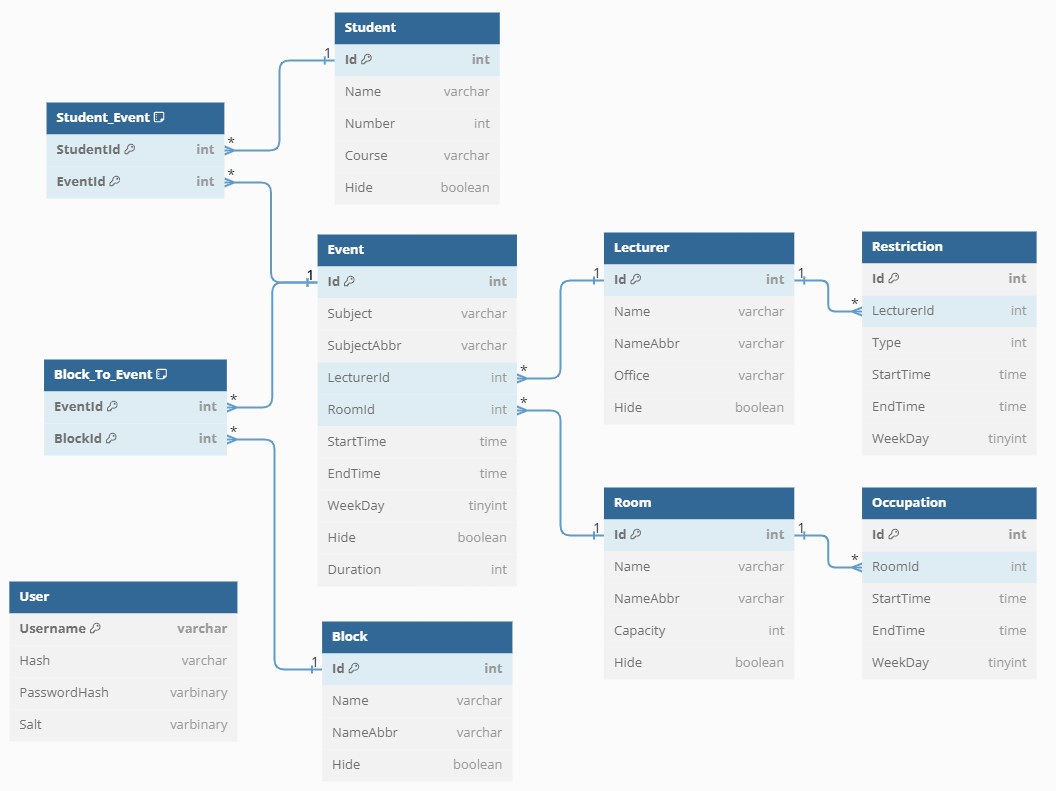
\includegraphics[width=1.1\columnwidth]{Development/uml.png}
%      \caption[UML]
%      {UML}
%      \label{fig:uml}
%\end{figure}